

% Set up the document
\documentclass[convert={density=300,size=1080x800,outext=.png}]{standalone}

% Include any extra LaTeX packages required
%\usepackage[square, numbers, comma, sort&compress]{natbib}  % Use the "Natbib" style for the references in the Bibliography

\usepackage{verbatim}  % Needed for the "comment" environment to make LaTeX comments
\usepackage[table,x11names]{xcolor} % needed for highlighted rows

\usepackage{tabularx,booktabs,adjustbox} % For tables
\usepackage{pdflscape} % For writing some pages in landscape mode
\usepackage{afterpage} % For control over the positioning of figures and tables.

% For pictures
\usepackage{tikz}
\usetikzlibrary{calc,fit,arrows,decorations.pathmorphing,backgrounds,fit,positioning}
\usetikzlibrary{shapes.symbols}

% tikz colour settings
\tikzset{pop0/.style={red!50!yellow},pop1/.style={violet!80},pop2/.style={olive!70!green}}

%% ----------------------------------------------------------------
\begin{document}
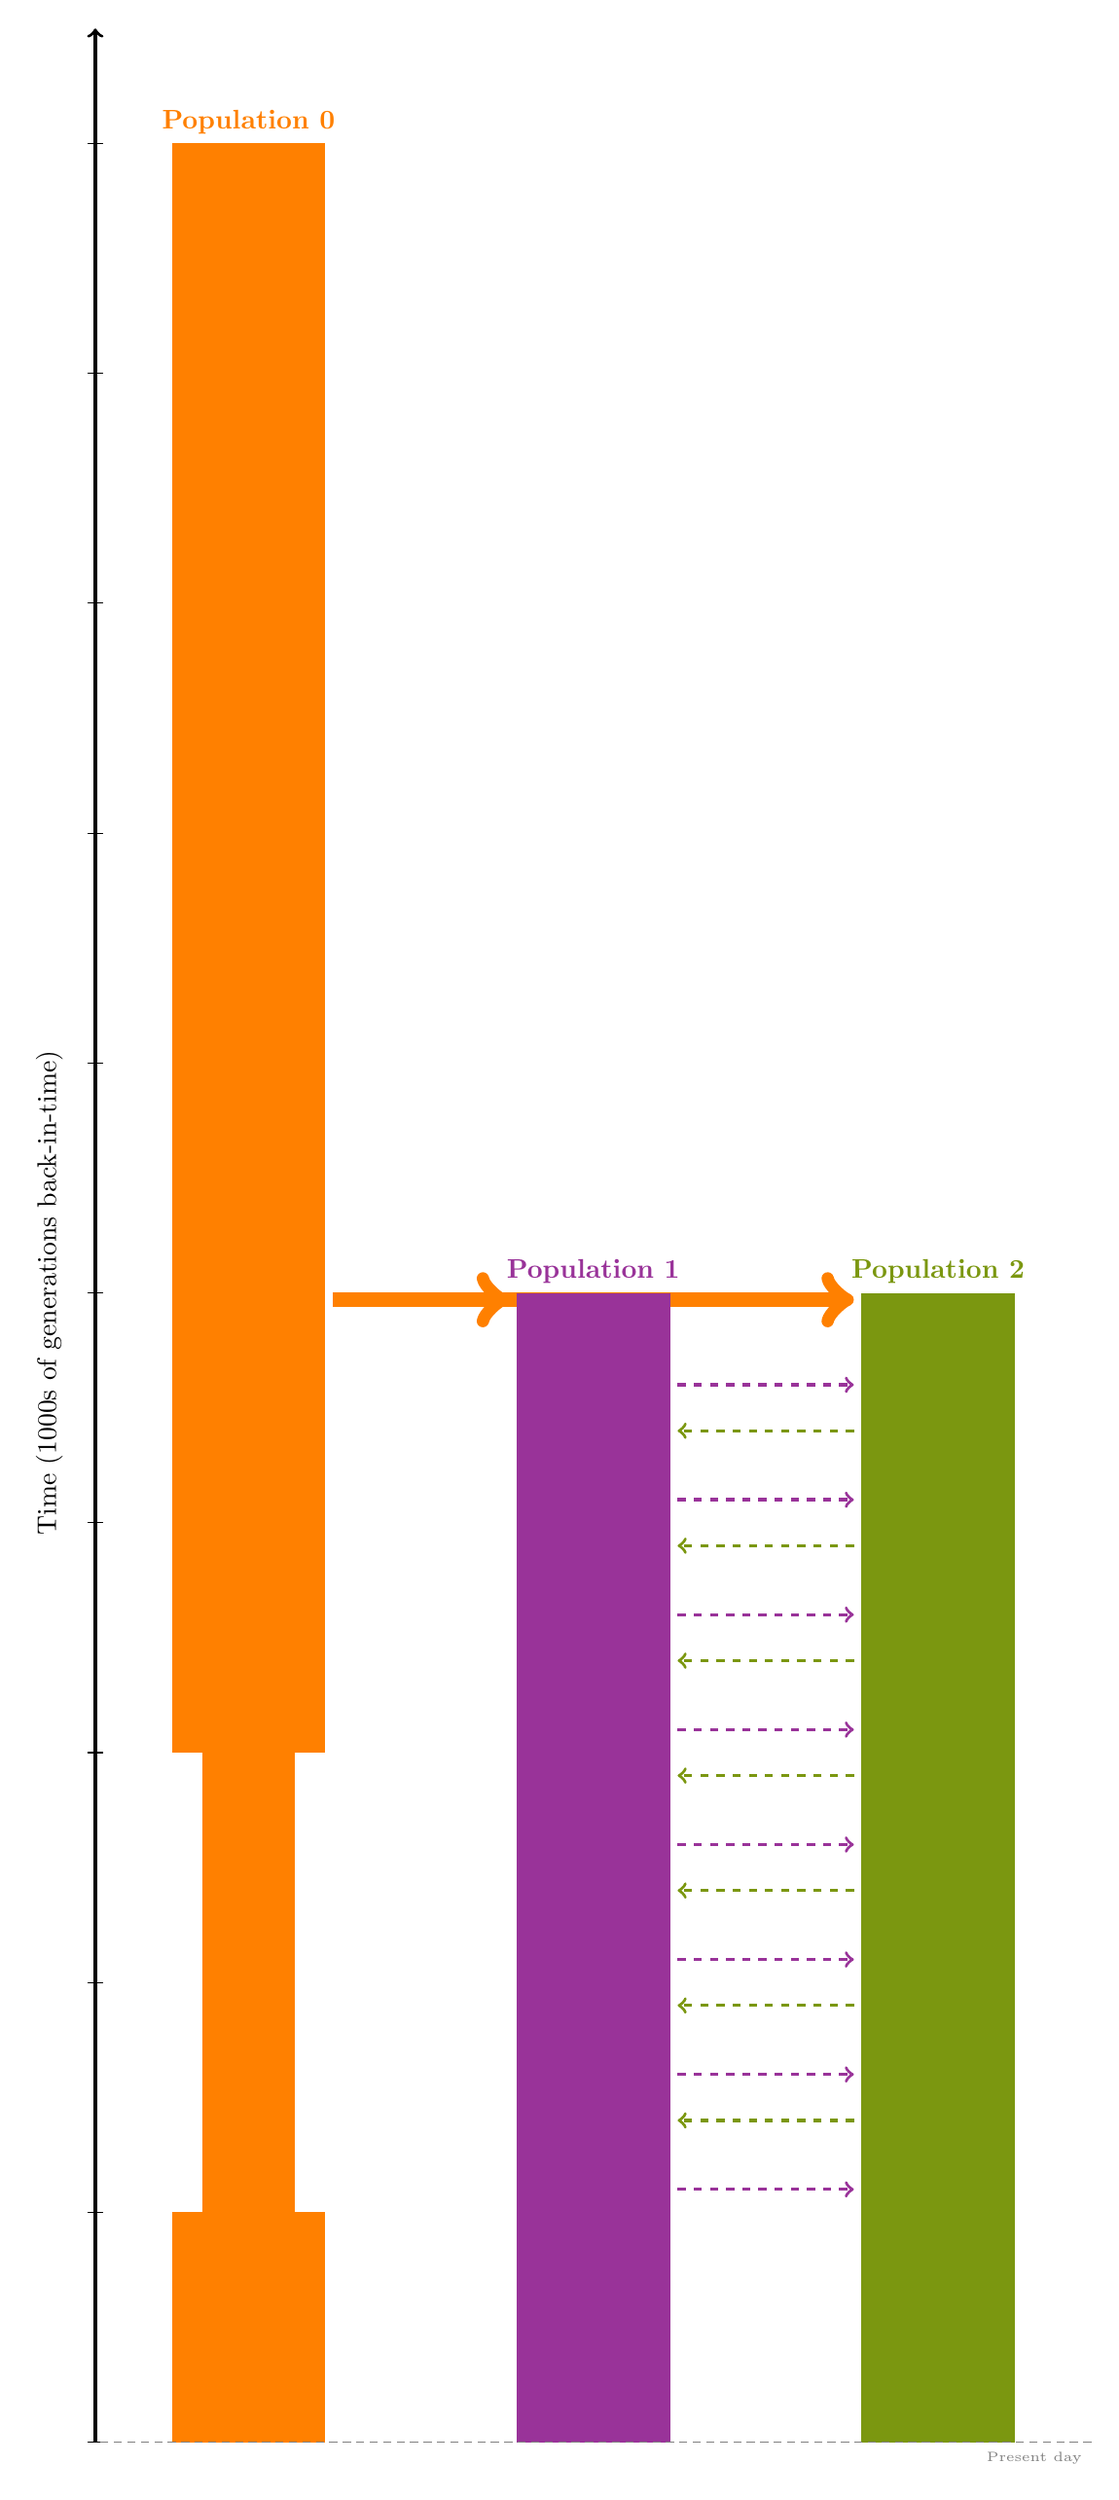
\begin{tikzpicture}[node distance=5mm and 5mm, yscale=3]

\tikzset{greynode/.style={font=\footnotesize,node distance=1cm and 1 cm,fill=black!10,draw=black!30,inner sep=0pt,minimum size=3.5mm,shape=circle},
mutations/.style={shape=starburst,fill=red!50!blue,inner sep=0.8pt,starburst points=11,starburst point height=.2cm}}

% Nodes
\node (origin) at (0,0){};
\node (pop0) at (1,0){};
\node (pop1) at (5.5,0){};
\node (pop2) at (10,0){};
\node (popwidth) at (2,0){};

% Axis
\node (leftAx) at (-1,0) {};
\draw[very thick,->] (-1,0) -- +(0, 10.5);
\foreach \y in {0, 1, 2, 3, 4, 5, 6, 7, 8, 9, 10} \draw ($(leftAx) + (-0.1, \y)$) -- ($(leftAx) + (0.1, \y)$); % tick marks
%\node[anchor=east] at ($(leftAx)$) {0}; \node[anchor=east] at ($(leftAx) + (0,5)$) {5};
\node[rotate=90,anchor=south] (leftLabel) at ($(leftAx) + (-0.3,5)$) {$\textrm{Time (1000s of generations back-in-time)}$};

% Migrations
\foreach \y in {0.5,1,1.5,2,2.5,3,3.5,4} \draw[pop1,dashed,->,very thick] ($(.1,.1) + (leftAx) + (0,\y + .5)+(pop1) + (popwidth)$) -- +(2.3,0);
\foreach \y in {1,1.5,2,2.5,3,3.5,4} \draw[pop2,dashed,->,very thick] ($(-.1,-.1) + (leftAx) + (0,\y + .5)+(pop2)$) -- +(-2.3,0);
\draw[pop0, ->, line width=2mm] ($(.1,0) + (leftAx) + (0,4.97)+(pop0) + (popwidth)$) -- +(2.3,0);
\draw[pop0, ->, line width=2mm] ($(.1,0) + (leftAx) + (0,4.97)+(pop0) + 2*(popwidth)$) -- +($2*(2.4,0)$);

% Populations
\foreach \x in {0} \fill[pop\x] ($(leftAx) + (pop\x)$) -- ++(0,10) -- ++(2, 0) -- ++(0, -10) -- cycle;
\foreach \x in {1, 2} \fill[pop\x] ($(leftAx) + (pop\x)$) -- ++(0,5) -- ++(2, 0) -- ++(0, -5) -- cycle;
\foreach \x in {0} \node[above,pop\x] (label\x) at ($(leftAx) + (pop\x) + (1, 10)$) {\bf Population \x};
\foreach \x in {1,2} \node[above,pop\x] (label\x) at ($(leftAx) + (pop\x) + (1, 5)$) {\bf Population \x};

% Times
\draw[densely dashed,color=gray] (12,0) node[below left] {\tiny Present day} -- (-1,0);

% White squares over pop0 bottleneck areas.
\fill[white] ($(leftAx) + 0.9*(pop0) + (0,1)$) -- ++($0.5*(pop0)$) -- ++(0,2) -- ++($-0.5*(pop0)$) -- cycle;
\fill[white] ($(leftAx) + 1.1*(pop0) +(popwidth) + (0,1)$) -- ++($-0.5*(pop0)$) -- ++(0,2) -- ++($0.5*(pop0)$) -- cycle;

\end{tikzpicture} 
\end{document}  % The End
%% ----------------------------------------------------------------